% 1986 年上海卷文史类第 6 题：正方体与两个截面
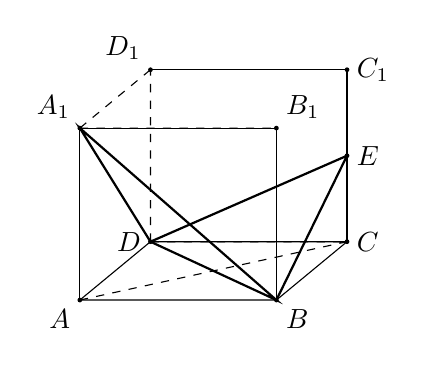
\begin{tikzpicture}[scale=0.78,>=stealth]
  \coordinate (A)  at (0,0);
  \coordinate (B)  at (3.2,0);
  \coordinate (C)  at (4.35,0.95);
  \coordinate (D)  at (1.15,0.95);
  \coordinate (A1) at (0,2.8);
  \coordinate (B1) at (3.2,2.8);
  \coordinate (C1) at (4.35,3.75);
  \coordinate (D1) at (1.15,3.75);
  \coordinate (E)  at (4.35,2.35);

  \draw (A)--(B)--(C)--(D)--cycle;
  \draw (A)--(A1)--(B1)--(B);
  \draw (B)--(B1);
  \draw (C)--(C1)--(D1);
  \draw[dashed] (D)--(D1) (A1)--(D1) (A1)--(B1);
  \draw[dashed] (D)--(C) (A)--(C);

  \draw[thick] (A1)--(B)--(D)--cycle;
  \draw[thick] (E)--(B) (E)--(D);
  \draw[dashed] (C)--(E);

  \fill (A) circle (1.1pt) node[below left] {$A$};
  \fill (B) circle (1.1pt) node[below right] {$B$};
  \fill (C) circle (1.1pt) node[right] {$C$};
  \fill (D) circle (1.1pt) node[left] {$D$};
  \fill (A1) circle (1.1pt) node[above left] {$A_1$};
  \fill (B1) circle (1.1pt) node[above right] {$B_1$};
  \fill (C1) circle (1.1pt) node[right] {$C_1$};
  \fill (D1) circle (1.1pt) node[above left] {$D_1$};
  \fill (E) circle (1.1pt) node[right] {$E$};
\end{tikzpicture}
